\begin{abwframe}
\node[anchor=north west,inner sep=0pt,outer sep=0pt] at (40.625,-55.791) {\begin{minipage}[t][69.584bp][c]{878.75bp}\setlength{\parindent}{0pt}\setlength{\parskip}{0pt}{\TimesNR\fontsize{44}{49.28}\selectfont\color{cBC0031}\bfseries\raggedright Universal Approximation Theorem\par}\end{minipage}};
\node[anchor=north west,inner sep=0pt,outer sep=0pt] at (40.625,-158.857) {\begin{minipage}[t][68.174bp][c]{884.89bp}\setlength{\parindent}{0pt}\setlength{\parskip}{0pt}{\TimesNR\fontsize{24}{26.88}\selectfont\color{c000000}\raggedright “A feedforward network with a single hidden layer single decision tree is sufficient to represent any function”\par}\end{minipage}};
\node[anchor=north west,inner sep=0pt,outer sep=0pt] at (508.35,-229.768) {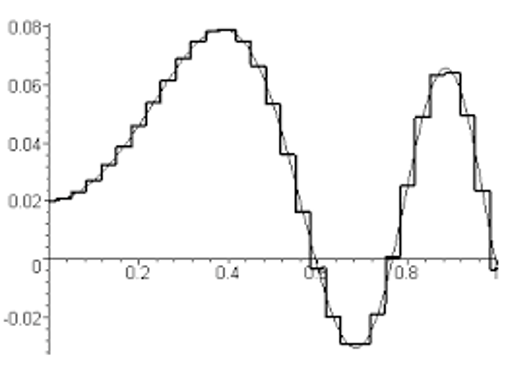
\includegraphics[width=379.885bp,height=280.53bp]{assets/source/slide-45-object-003.png}};
\draw[fill=cBC0031,fill opacity=1,draw=c890021,line width=1bp,rotate around={0:(281.553,-245.78)}] (281.553,-245.78) ellipse [x radius=22.68bp,y radius=22.667bp];
\node[anchor=north west,inner sep=0pt,outer sep=0pt] at (182.453,-257.615) {\begin{minipage}[t][40.905bp][t]{48.402bp}\setlength{\parindent}{0pt}\setlength{\parskip}{0pt}{\TimesNR\fontsize{18}{20.16}\selectfont\color{c000000}\itshape\raggedright \ensuremath{x}< 1 2 \par}\end{minipage}};
\draw[fill=none,draw=c1F1D21,line width=0.5bp,-{Stealth}] (196.504,-261.808) -- (265.516,-326.157);
\draw[fill=cBC0031,fill opacity=1,draw=c890021,line width=1bp,rotate around={0:(196.504,-348.823)}] (196.504,-348.823) ellipse [x radius=22.68bp,y radius=22.667bp];
\draw[fill=none,draw=c1F1D21,line width=0.5bp,-{Stealth}] (297.59,-261.808) -- (366.602,-326.17);
\draw[fill=cBC0031,fill opacity=1,draw=c890021,line width=1bp,rotate around={0:(366.602,-348.837)}] (366.602,-348.837) ellipse [x radius=22.68bp,y radius=22.667bp];
\node[anchor=north west,inner sep=0pt,outer sep=0pt] at (329.689,-257.615) {\begin{minipage}[t][40.905bp][t]{48.402bp}\setlength{\parindent}{0pt}\setlength{\parskip}{0pt}{\TimesNR\fontsize{18}{20.16}\selectfont\color{c000000}\itshape\raggedright \ensuremath{x}\ensuremath{\ge} 1 2 \par}\end{minipage}};
\draw[fill=none,draw=c1F1D21,line width=0.5bp,-{Stealth}] (152.658,-364.851) -- (180.467,-430.303);
\draw[fill=cBC0031,fill opacity=1,draw=c890021,line width=1bp,rotate around={0:(152.658,-452.969)}] (152.658,-452.969) ellipse [x radius=22.68bp,y radius=22.667bp];
\draw[fill=none,draw=c1F1D21,line width=0.5bp,-{Stealth}] (212.541,-364.851) -- (233.871,-431.378);
\draw[fill=cBC0031,fill opacity=1,draw=c890021,line width=1bp,rotate around={0:(233.871,-454.044)}] (233.871,-454.044) ellipse [x radius=22.68bp,y radius=22.667bp];
\node[anchor=north west,inner sep=0pt,outer sep=0pt] at (118.222,-356.929) {\begin{minipage}[t][40.905bp][t]{48.402bp}\setlength{\parindent}{0pt}\setlength{\parskip}{0pt}{\TimesNR\fontsize{18}{20.16}\selectfont\color{c000000}\itshape\raggedright \ensuremath{x}< 1 4 \par}\end{minipage}};
\node[anchor=north west,inner sep=0pt,outer sep=0pt] at (218.391,-356.07) {\begin{minipage}[t][40.905bp][t]{48.402bp}\setlength{\parindent}{0pt}\setlength{\parskip}{0pt}{\TimesNR\fontsize{18}{20.16}\selectfont\color{c000000}\itshape\raggedright \ensuremath{x}\ensuremath{\ge} 1 4 \par}\end{minipage}};
\draw[fill=none,draw=c1F1D21,line width=0.5bp,-{Stealth}] (323.244,-364.864) -- (350.565,-430.496);
\draw[fill=cBC0031,fill opacity=1,draw=c890021,line width=1bp,rotate around={0:(323.244,-453.162)}] (323.244,-453.162) ellipse [x radius=22.68bp,y radius=22.667bp];
\draw[fill=none,draw=c1F1D21,line width=0.5bp,-{Stealth}] (382.638,-364.864) -- (404.457,-431.571);
\draw[fill=cBC0031,fill opacity=1,draw=c890021,line width=1bp,rotate around={0:(404.457,-454.237)}] (404.457,-454.237) ellipse [x radius=22.68bp,y radius=22.667bp];
\node[anchor=north west,inner sep=0pt,outer sep=0pt] at (288.753,-356.07) {\begin{minipage}[t][40.905bp][t]{48.402bp}\setlength{\parindent}{0pt}\setlength{\parskip}{0pt}{\TimesNR\fontsize{18}{20.16}\selectfont\color{c000000}\itshape\raggedright \ensuremath{x}< 3 4 \par}\end{minipage}};
\node[anchor=north west,inner sep=0pt,outer sep=0pt] at (396.925,-356.929) {\begin{minipage}[t][40.905bp][t]{48.402bp}\setlength{\parindent}{0pt}\setlength{\parskip}{0pt}{\TimesNR\fontsize{18}{20.16}\selectfont\color{c000000}\itshape\raggedright \ensuremath{x}\ensuremath{\ge} 3 4 \par}\end{minipage}};
\node[anchor=north west,inner sep=0pt,outer sep=0pt] at (130.428,-500.769) {\begin{minipage}[t][21.881bp][t]{38.386bp}\setlength{\parindent}{0pt}\setlength{\parskip}{0pt}{\TimesNR\fontsize{18}{20.16}\selectfont\color{c000000}\itshape\raggedright 0.03\par}\end{minipage}};
\node[anchor=north west,inner sep=0pt,outer sep=0pt] at (213.491,-500.769) {\begin{minipage}[t][21.881bp][t]{38.385bp}\setlength{\parindent}{0pt}\setlength{\parskip}{0pt}{\TimesNR\fontsize{18}{20.16}\selectfont\color{c000000}\itshape\raggedright 0.07\par}\end{minipage}};
\node[anchor=north west,inner sep=0pt,outer sep=0pt] at (300.093,-499.855) {\begin{minipage}[t][21.881bp][t]{52.017bp}\setlength{\parindent}{0pt}\setlength{\parskip}{0pt}{\TimesNR\fontsize{18}{20.16}\selectfont\color{c000000}\itshape\raggedright \ensuremath{-}0.01\par}\end{minipage}};
\node[anchor=north west,inner sep=0pt,outer sep=0pt] at (388.244,-501.782) {\begin{minipage}[t][21.881bp][t]{38.385bp}\setlength{\parindent}{0pt}\setlength{\parskip}{0pt}{\TimesNR\fontsize{18}{20.16}\selectfont\color{c000000}\itshape\raggedright 0.05\par}\end{minipage}};
\node[anchor=north west,inner sep=0pt,outer sep=0pt] at (56.693,-499.702) {\begin{minipage}[t][11.952bp][c]{324bp}\setlength{\parindent}{0pt}\setlength{\parskip}{0pt}{\TimesNR\fontsize{10}{11.2}\selectfont\color{c7F7F7F}\raggedright Analytics for a Better World Lecture 2\par}\end{minipage}};
\node[anchor=north west,inner sep=0pt,outer sep=0pt] at (880.898,-499.702) {\begin{minipage}[t][11.952bp][c]{22.409bp}\setlength{\parindent}{0pt}\setlength{\parskip}{0pt}{\TimesNR\fontsize{10}{11.2}\selectfont\color{c7F7F7F}\bfseries\raggedleft 45\par}\end{minipage}};
\end{abwframe}
